\section{(9 points)}

\subsection{(4 points)}

Entre le $1^{er}$ janvier 2014 et le 31 décembre 2014, une clinique enregistre \num{1200} accouchements. Depuis quelques années, le nombre annuel d'accouchements a augmenté de 3 \% par an. L'objectif du directeur de la clinique est d'atteindre les \num{8000} accouchements réalisés dans la clinique d'ici fin 2020, en supposant que ce pourcentage d'augmentation moyen reste constant.\\

Pour tout nombre entier naturel $n$, on note $u_n$ le nombre annuel d'accouchements dans cette clinique pour l'année $2014+n$. Ainsi $u_0$ est le nombre d'accouchements durant l'année 2014, et $u_0=\num{1200}$.

\begin{questions}
	\question[\half] Déterminer le nombre d'accouchements  qui ont eu lieu dans cette clinique en 2015.
	\begin{solution}
		Le coefficient multiplicateur correspondant à une augmentetion de 3\% est \num{1.03}.
		
		$1200 \times \num{1.03} = 1236$
		
		En 2015, il y a eu \num{1236} accouchements dans cette clinique.
	\end{solution}
	\question[1] Quelle est la nature de la suite $(u_n)$ ? Justifier et donner ses éléments caractéristiques.
	\begin{solution}
		Chaque année, le nombre de naissance augmente de 3\%, donc chaque terme de la suite est obtenu en multipliant le précédent par \num{1.03}. C'est une suite géométrique de terme initial $u_0 = 1200$ et de raison $q=\num{1.03}$.
	\end{solution}
	\question[1] Pour tout entier naturel $n$, exprimer $u_n$ en fonction de $n$.
	\begin{solution}
		Expression de $u_n$ en fonction de $n$ :
		
		\begin{eqnarray*}
			u_n &=& u_0 \times q^n \\
			u_n &=& \num{1200} \times \num{1.03}^n 
		\end{eqnarray*}
	\end{solution}

	\question[\half] Déterminer le nombre d'accouchements qui auront lieu dans cette clinique en 2017 selon ce modèle. On arrondira ce résultat à l'unité.
	\begin{solution}
		$2017 - 2014 = 3$, calcul de $u_3$ :
		
		\begin{eqnarray*}
			u_3 &=& \num{1200} \times \num{1.03}^3 \\
			u_3 & \approx & \num{1311}
		\end{eqnarray*}
	
	En 2017, il y aura \num{1311} accouchements.
	\end{solution}
	\question[1] On rappelle le résultat suivant :
	
	Si $(u_n)$ est une suite géométrique de premier terme $u_0$ et de raison $q$, $q\neq1$, alors :
	\begin{equation*}
		u_0 + u_1 + u_2 + ... + u_n = u_o \times \dfrac{1-q^{n+1}}{1-q}
	\end{equation*}

	\begin{parts}
		\part[] Déterminer le nombre total d'accouchements qui auront lieu dans cette clinique entre le $1^{er}$ janvier 2014 et el 31 décembre 2020. On arrondira le résultat à l'unité.
		\begin{solution}
			
			2020 est l'année de rang 6, calcul de $S_{6}$:
			\begin{eqnarray*}
				S_{6} &=& 1200 \times \dfrac{1 - \num{1.03}^7}{1 - 1\num{1.03}} \\
				S_{6} & \approx & \num{9195}
			\end{eqnarray*}
		
		Selon ce modèle, il y aura \num{9195} accouchements dans cette clinique entre 2014 et 2020.
		\end{solution}
		\part[] Selon ce modèle, le directeur peut-il espérer atteindre son objectif ? Justifier.
		\begin{solution}
			9195 est supérieur à 8000, donc le directeur peut atteindre son objectif.
		\end{solution}
		
	\end{parts}
\end{questions}

\subsection{(5 points)}

L'Organisation Mondiale de la Santé (OMS) recommande un taux maximum de 15 \% de césariennes pour ce type de clinique. En France, les experts estiment que le taux de césariennes est anormal s'il dépasse les 25 \%.\\

Un journal régional a mené une enquête auprès d'un certain nombre de femmes ayant accouché dans la clinique en 2014. L'objectif de cette étude était de déterminer si la clinique avait tendance à recourir trop fréquemment à une césarienne sans réelle justification médicale. Lors de cette enquête, le journaliste a obtenu les résultats suivants :

\begin{itemize}
	\item 43 \% des femmes interrogées sont primipares (c'est-à-dire qu'il s'agit de leur premier enfant) et parmi elles, 23 \% ont accouché par césarienne à la clinique.
	\item 11 \% des femmes interrogées sont des multipares (c'est-à-dire qu'elles ont déjà accouché auparavant) ayant accouché par césarienne lors d'un accouchement précédent et parmi elles, 64 \% ont accouché par césarienne à la clinique.
	\item Les autres sont de multipares n'ayant jamais accouché par césarienne auparavant et parmi elles, 8 \% ont accouché par césarienne à la clinique.	
\end{itemize}

On choisit au hasard une femme ayant participé à l'enquête.
On considère les événements suivants :
\begin{itemize}
	\item[$A_0$ :]  <<La femme est une primipare >> (c'est-à-dire qu'il s'agit de son premier enfant);
	\item[$M_1$ :]  <<La femme est une multipare qui a déjà accouché par césarienne >> ;
	\item[$M_2$ :]  <<La femme est une multipare qui n'a jamais accouché par césarienne auparavant>> ;
	\item[$C$ :] <<La femme a accouché par césarienne à la clinique>>.
\end{itemize}

L'événement contraire de l'événement $C$ est noté $\bar{C}$.

\begin{questions}
	\question[1] \'A partir des données de l'énoncé, déterminer :
		\begin{parts}
			\part[\half] La probabilité de l'événement $M_1$, notée $P(M_1)$;
			\begin{solution}
				$P(M_1) = \frac{11}{100} = \num{0.11}$
			\end{solution}
			\part[\half] La probabilité que la femme ait accouché par césarienne sachant qu'elle est une multipare qui a déjà accouché par césarienne, notée $P_{M_1}(C)$.
			\begin{solution}
				$P_{M_1}(C) = \frac{64}{100} = \num{0.64}$
			\end{solution}
		\end{parts}
	
	\question[1] Recopier et compléter l'arbre ci-dessous :
	
		
% Set the overall layout of the tree
\tikzstyle{level 1}=[level distance=3.5cm, sibling distance=3.5cm]
\tikzstyle{level 2}=[level distance=3.5cm, sibling distance=2cm]

% Define styles for bags and leafs
\tikzstyle{bag} = [text width=4em, text centered]
\tikzstyle{end} = [circle, minimum width=3pt,fill, inner sep=0pt]

% The sloped option gives rotated edge labels. Personally
% I find sloped labels a bit difficult to read. Remove the sloped options
% to get horizontal labels. 
\begin{tikzpicture}[grow=right, sloped]
\node[bag] {}
    child {
        node[bag] {$M_2$}        
            child {
                node[end, label=right:
                    {$\bar{C}$ }] {}
                edge from parent
                node[below] {...}
                %node[below]  {$\frac{4}{9}$}
            }
            child {
                node[end, label=right:
                    {$C$}] {}
                edge from parent
                node[above] {...}
                %node[below]  {$\frac{5}{9}$}
            }
            edge from parent 
            %node[above] {$W$}
            node[below]  {}
    }
    child {
        node[bag] {$M_1$}        
        child {
                node[end, label=right:
                    {$\bar{C} $}] {}
                edge from parent
                %node[above] {$B$}
                node[below]  {...}
            }
            child {
                node[end, label=right:
                    {$C$}] {}
                edge from parent
                node[above] {...}
%                node[below]  {$\frac{6}{9}$}
            }
        edge from parent         
            %node[above] {$B$}
            node[above]  {...}
    }
    child {
    	node[bag] {$A_0$}        
    	child {
    		node[end, label=right:
    		{$\bar{C}$}] {}
    		edge from parent
    		%node[above] {$B$}
    		node[below]  {...}
    	}
    	child {
    		node[end, label=right:
    		{$C$}] {}
    		edge from parent
    		node[above] {...}
    		%                node[below]  {$\frac{6}{9}$}
    	}
    	edge from parent         
    	%node[above] {$B$}
    	node[above]  {...}
    };
\end{tikzpicture}

	
	\begin{solution}
			
% Set the overall layout of the tree
\tikzstyle{level 1}=[level distance=3.5cm, sibling distance=3.5cm]
\tikzstyle{level 2}=[level distance=3.5cm, sibling distance=2cm]

% Define styles for bags and leafs
\tikzstyle{bag} = [text width=4em, text centered]
\tikzstyle{end} = [circle, minimum width=3pt,fill, inner sep=0pt]

% The sloped option gives rotated edge labels. Personally
% I find sloped labels a bit difficult to read. Remove the sloped options
% to get horizontal labels. 
\begin{tikzpicture}[grow=right, sloped]
\node[bag] {}
    child {
        node[bag] {$M_2$}        
            child {
                node[end, label=right:
                    {$\bar{C}$ }] {}
                edge from parent
                node[below] {$0,92$}
                %node[below]  {$\frac{4}{9}$}
            }
            child {
                node[end, label=right:
                    {$C$}] {}
                edge from parent
                node[above] {$0,08$}
                %node[below]  {$\frac{5}{9}$}
            }
            edge from parent 
            %node[above] {$W$}
            node[below]  {$0,46$}
    }
    child {
        node[bag] {$M_1$}        
        child {
                node[end, label=right:
                    {$\bar{C} $}] {}
                edge from parent
                %node[above] {$B$}
                node[below]  {$0,36$}
            }
            child {
                node[end, label=right:
                    {$C$}] {}
                edge from parent
                node[above] {$0,64$}
%                node[below]  {$\frac{6}{9}$}
            }
        edge from parent         
            %node[above] {$B$}
            node[above]  {$0,11$}
    }
    child {
    	node[bag] {$A_0$}        
    	child {
    		node[end, label=right:
    		{$\bar{C}$}] {}
    		edge from parent
    		%node[above] {$B$}
    		node[below]  {$0,77$}
    	}
    	child {
    		node[end, label=right:
    		{$C$}] {}
    		edge from parent
    		node[above] {$0,23$}
    		%                node[below]  {$\frac{6}{9}$}
    	}
    	edge from parent         
    	%node[above] {$B$}
    	node[above]  {$0,43$}
    };
\end{tikzpicture}

	\end{solution}
%		\begin{center}
%			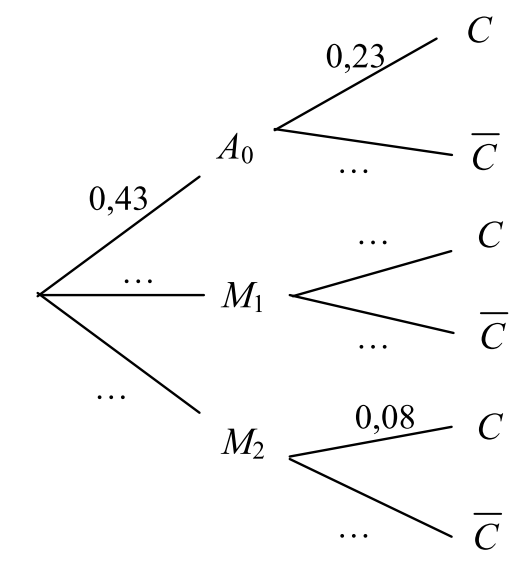
\includegraphics[scale=0.4]{img/arbre}
%		\end{center}	
	
	\question[1] Définir par une phrase l'événement $A_0 \cap C$ puis calculer la probabilité $P(A_0 \cap C)$.
	\begin{solution}
		$A_0 \cap C$ : <<La femme est une primipare et elle a accouché par césarienne à la clinique.>>
		
		\begin{eqnarray*}
			P(A_0 \cap C) &=& \num{0.43} \times \num{0.23} \\
			P(A_0 \cap C) &=& \num{0.0989}
		\end{eqnarray*}
	\end{solution}
	
	\question[1] Montrer que la probabilité qu'une femme accouche par césarienne dans cette clinique est égale à \num{0.2061}.
	\begin{solution}
		Calcul de $P(M_1 \cap C)$ et $P(M_2 \cap C)$.
		
		\begin{eqnarray*}
			P(M_1 \cap C) &=& \num{0.11} \times \num{0.64} \\
			P(M_1 \cap C) &=& \num{0.0704} \\
			& & \\
			P(M_2 \cap C) &=& \num{0.08} \times \num{0.23} \\
			P(M_2 \cap C) &=& \num{0.0368} 			
		\end{eqnarray*}
	
	Calcul de $P(C)$ :
	\begin{eqnarray*}
		P(C) &=& P(A_0 \cap C) + P(M_1 \cap C) + P(M_2 \cap C) \\
		P(C) &=& \num{0.0989} + \num{0.0704} + \num{0.0368} \\
		P(C) &=& 0.2061				
	\end{eqnarray*}
	\end{solution}
	
	\question[1] La clinique étudiée respecte-t-elle les recommandations de l'OMS ? Des experts français ?
	\begin{solution}
		Dans cette clinique, le taux de césarienne est de \num{20.61} \%, donc elle respecte les recommandations des experts français mais pas celles de l'OMS. 
	\end{solution}
		
\end{questions}